\section{SVM-классификация}
\subsection{Постановка задачи}
\par Метод опорных векторов (Support Vector Machine, SVM) решает задачу бинарной классификации, где требуется найти оптимальную гиперплоскость, разделяющую два класса в пространстве признаков. Оптимальность понимается как максимизация ширины разделяющей полосы между классами.

\subsection{Математическая формализация}
\par Пусть дана обучающая выборка \( \{(x_i, y_i)\}_{i=1}^{\ell} \), где \( x_i \in \mathbb{R}^n \) - векторы признаков, \( y_i \in \{-1,+1\} \) - метки классов. Разделяющая гиперплоскость описывается уравнением:
\begin{equation*}
    \langle w,x \rangle - w_0 = 0,
\end{equation*}
где \( w \in \mathbb{R}^n \) - вектор весов, \( w_0 \in \mathbb{R} \) - порог.

\subsection{Условия разделимости}
\par Для корректной классификации должны выполняться условия:
\begin{equation*}
    \begin{cases}
        \langle w,x_i \rangle - w_0 \geq +1, & \text{если } y_i = +1 \\
        \langle w,x_i \rangle - w_0 \leq -1, & \text{если } y_i = -1
    \end{cases}
\end{equation*}
\par Эти условия можно объединить:
\begin{equation*}
    y_i(\langle w,x_i \rangle - w_0) \geq 1, \quad i = 1,\ldots,\ell
\end{equation*}

\subsection{Оптимизационная задача}
\par Ширина разделяющей полосы равна \( \frac{2}{\|w\|} \). Задача максимизации ширины эквивалентна задаче минимизации:
\begin{equation*}
    \frac{1}{2}\|w\|^2 \to \min_{w,w_0}
\end{equation*}
при ограничениях \( y_i(\langle w,x_i \rangle - w_0) \geq 1 \).

\subsection{Двойственная задача}
\par Применяя метод множителей Лагранжа, получаем двойственную задачу:
\begin{equation*}
    L(w,w_0,\lambda) = \frac{1}{2}\|w\|^2 - \sum_{i=1}^{\ell} \lambda_i(y_i(\langle w,x_i \rangle - w_0) - 1)
\end{equation*}
\par Условия оптимальности:
\begin{equation*}
    \begin{cases}
        w = \sum_{i=1}^{\ell} \lambda_i y_i x_i \\
        \sum_{i=1}^{\ell} \lambda_i y_i = 0
    \end{cases}
\end{equation*}

\subsection{Ядра}
\par Для нелинейной классификации используется переход в пространство признаков большей размерности через отображение \( \phi(x) \). Скалярное произведение заменяется на ядро:
\begin{equation*}
    K(x,z) = \langle \phi(x),\phi(z) \rangle
\end{equation*}
\par Популярные ядра:
\begin{itemize}
    \item Линейное: \( K(x,z) = \langle x,z \rangle \)
    \item Полиномиальное: \( K(x,z) = (\langle x,z \rangle + 1)^d \)
    \item RBF: \( K(x,z) = \exp(-\gamma\|x-z\|^2) \)
\end{itemize}

\subsection{Дискриминантная функция в ядровом пространстве}
\par После применения ядрового преобразования классификация новых точек осуществляется с помощью дискриминантной функции, которая принимает вид:
\begin{equation*}
    f(x) = \sum_{i=1}^{\ell} \lambda_i y_i K(x_i,x) - w_0
\end{equation*}
где:
\begin{itemize}
    \item \(x_i\) - опорные векторы из обучающей выборки
    \item \(\lambda_i\) - множители Лагранжа (двойственные переменные)
    \item \(y_i\) - метки классов опорных векторов
    \item \(K(x_i,x)\) - значение ядровой функции между опорным вектором и классифицируемой точкой
    \item \(w_0\) - порог, определяющий сдвиг разделяющей гиперплоскости
\end{itemize}

\par Важно отметить, что в этой формуле суммирование происходит только по опорным векторам, так как для остальных точек обучающей выборки \(\lambda_i = 0\). Это свойство обеспечивает эффективность вычислений при классификации новых точек.

\par Решающее правило для определения класса новой точки:
\begin{equation*}
    \text{class}(x) = \text{sign}(f(x)) = 
    \begin{cases}
        +1, & \text{если } f(x) > 0 \\
        -1, & \text{если } f(x) < 0
    \end{cases}
\end{equation*}

\subsection{Мягкие границы}
\par Для случая линейно неразделимой выборки вводятся переменные ослабления \( \xi_i \geq 0 \):
\begin{equation*}
    y_i(\langle w,x_i \rangle - w_0) \geq 1 - \xi_i
\end{equation*}
\par Целевая функция модифицируется:
\begin{equation*}
    \frac{1}{2}\|w\|^2 + C\sum_{i=1}^{\ell} \xi_i \to \min_{w,w_0,\xi}
\end{equation*}
где \( C > 0 \) - параметр регуляризации.

\subsection{Задача 1}
\textbf{Условие:} 
\par Дан набор точек в двумерном пространстве с метками классов:
\begin{equation*}
    \begin{array}{ll}
        x_1 = (0,0), & y_1 = -1 \\
        x_2 = (2,0), & y_2 = +1 \\
        x_3 = (0,2), & y_3 = +1 \\
        x_4 = (2,2), & y_4 = +1
    \end{array}
\end{equation*}
\par В результате обучения SVM с линейным ядром получены следующие значения двойственных переменных:
\begin{equation*}
    \lambda_1 = 0.5, \quad \lambda_2 = 0, \quad \lambda_3 = 0.5, \quad \lambda_4 = 0
\end{equation*}
\par Найдите вектор весов \(w\) и определите, является ли точка \(x_{\text{new}} = (1,1)\) опорным вектором, если известно, что она лежит точно на разделяющей гиперплоскости.

\textbf{Решение:}
\par 1. Найдем вектор весов \(w\) через опорные векторы:
\begin{equation*}
    w = \sum_{i=1}^4 \lambda_i y_i x_i
\end{equation*}

\par 2. Подставляем известные значения:
\begin{align*}
    w &= 0.5 \cdot (-1) \cdot (0,0) + 0 \cdot (+1) \cdot (2,0) + \\
    &+ 0.5 \cdot (+1) \cdot (0,2) + 0 \cdot (+1) \cdot (2,2) \\
    &= (0,0) + (0,0) + (0,0.6) + (0,0) \\
    &= (0,1)
\end{align*}

\par 3. Для точек на разделяющей гиперплоскости выполняется:
\begin{equation*}
    \langle w,x \rangle - w_0 = 0
\end{equation*}

\par 4. Подставляя координаты \(x_{\text{new}} = (1,1)\):
\begin{equation*}
    \langle (0,1),(1,1) \rangle - w_0 = 0
\end{equation*}
\begin{equation*}
    w_0 = 1
\end{equation*}

\par 5. Чтобы точка была опорным вектором, она должна лежать на границе разделяющей полосы, то есть:
\begin{equation*}
    y_{\text{new}}(\langle w,x_{\text{new}} \rangle - w_0) = \pm 1
\end{equation*}

\par 6. Проверяем это условие:
\begin{equation*}
    \langle (0,1),(1,1) \rangle - 1 = 0
\end{equation*}
Получаем 0, что не равно $\pm1$.

\textbf{Ответ:} \(w = (0,1)\). Точка \(x_{\text{new}}\) не является опорным вектором.

\subsection{Задача 2}
\textbf{Условие:} 
\par Дано множество точек в двумерном пространстве:
\begin{equation*}
    \begin{array}{ll}
        x_1 = (1,1), & y_1 = +1 \\
        x_2 = (2,2), & y_2 = +1 \\
        x_3 = (0,0), & y_3 = -1 \\
        x_4 = (-1,1), & y_4 = -1
    \end{array}
\end{equation*}
\par После обучения SVM получена разделяющая гиперплоскость \(2/3 \cdot x_{i1} + 1/3 \cdot x_{i2} - 1 = 0\). Определите, какие из точек являются опорными векторами.

\textbf{Решение:}
\par Опорными векторами являются точки, лежащие на границе разделяющей полосы. Для их определения нужно:

\par 1. Запишем вектор весов из уравнения гиперплоскости:
\begin{equation*}
    w = (2/3,1/3) \quad w_0 = 1
\end{equation*}

\par 2. Вычислим отступ для каждой точки по формуле:
\begin{equation*}
    M(x) = y(\langle w,x \rangle - w_0) = y(2x_{i1} + x_{i2} - 3)
\end{equation*}

\par 3. Проверяем каждую точку:
\begin{align*}
    M(x_1) &= (+1)(2/3 \cdot 1 + 1/3 \cdot 1 - 1) = 0 \\
    M(x_2) &= (+1)(2/3 \cdot 2 + 1/3 \cdot 2 - 1) = 1 \\
    M(x_3) &= (-1)(2/3 \cdot 0 + 1/3 \cdot 0 - 1) = 1 \\
    M(x_4) &= (-1)(2/3 \cdot (-1) + 1/3 \cdot 1 - 1) = 4/3
\end{align*}

\par 4. Опорными векторами являются точки с отступом, равным единице, а также точки, лежащие на разделяющей гиперплоскости (отступ равен нулю).

\textbf{Ответ:} Точки \(x_2\) и \(x_3\) являются опорными векторами.

\subsection{Задача 3}
\textbf{Условие:} 
\par При обучении SVM с полиномиальным ядром второй степени \(K(x,z) = (\langle x,z \rangle + 1)^2\) получены следующие опорные векторы:
\begin{equation*}
    \begin{array}{ll}
        x_1 = (2,0), & \lambda_1 = 0.2, \quad y_1 = +1 \\
        x_2 = (0,1), & \lambda_2 = 0.3, \quad y_2 = -1 \\
        x_3 = (1,1), & \lambda_3 = 0.1, \quad y_3 = +1
    \end{array}
\end{equation*}
\par К какому классу будет отнесена точка \(x_{\text{new}} = (1,0)\), если \(w_0 = 0.5\)?

\textbf{Решение:}
\par Для определения класса точки нужно найти знак дискриминантной функции:
\begin{equation*}
    f(x) = \sum_{i=1}^3 \lambda_i y_i K(x_i,x) - w_0
\end{equation*}

\par Вычислим значения ядра для \(x_{\text{new}}\) и каждого опорного вектора:
\begin{align*}
    K(x_1,x_{\text{new}}) &= (2 \cdot 1 + 0 \cdot 0 + 1)^2 = 9 \\
    K(x_2,x_{\text{new}}) &= (0 \cdot 1 + 1 \cdot 0 + 1)^2 = 1 \\
    K(x_3,x_{\text{new}}) &= (1 \cdot 1 + 1 \cdot 0 + 1)^2 = 4
\end{align*}

\par Подставляем в дискриминантную функцию:
\begin{align*}
    f(x_{\text{new}}) &= 0.2 \cdot (+1) \cdot 9 + 0.3 \cdot (-1) \cdot 1 + 0.1 \cdot (+1) \cdot 4 - 0.5 \\
    &= 1.8 - 0.3 + 0.4 - 0.5 = 1.4
\end{align*}

\par Так как \(f(x_{\text{new}}) > 0\), точка относится к классу +1.

\textbf{Ответ:} Точка \(x_{\text{new}}\) будет отнесена к классу +1.

\section{SVM-регрессия}
\subsection{Постановка задачи}
\par В задаче регрессии требуется найти функцию \( f(x) = w^T \phi(x) + b \), которая аппроксимирует целевые значения \( y \) на основе входных данных \( x \), минимизируя ошибки предсказания.
\par В SVM-регрессии вводится допустимая область погрешностей — \(\epsilon\)-окрестность. Это означает, что отклонения \( |f(x_i) - y_i| \) в пределах \(\epsilon\) считаются несущественными, и модель игнорирует их. Цель — минимизировать сложность модели, связанную с \(\|w\|\), штрафуя при этом за отклонения, выходящие за пределы \(\epsilon\).

\subsection{Прямая задача}
\par\textbf{Функция потерь.}  
Для задачи SVM-регрессии используется \(\epsilon\)-чувствительная функция потерь:
\begin{equation*}
    L_\epsilon(f(x), y) = 
    \begin{cases} 
        0, & \text{если } |f(x) - y| \leq \epsilon, \\ 
        |f(x) - y| - \epsilon, & \text{иначе.}
    \end{cases}
\end{equation*}
\noindent\textbf{Прямая постановка задачи:}
\begin{equation*}
    \min_{w, b} \frac{1}{2} \|w\|^2 + C \sum_{i=1}^n L_\epsilon(f(x_i), y_i),
\end{equation*}
где:
\begin{itemize}
    \item \(\|w\|^2\) — регуляризационный член, минимизирующий сложность модели,
    \item \(C\) — коэффициент, регулирующий баланс между штрафами за ошибки и сложностью модели,
    \item \(L_\epsilon(f(x_i), y_i)\) — штраф за выход за пределы \(\epsilon\)-окрестности.
\end{itemize}

\subsection{Преобразование задачи}
\par Для учёта отклонений выше \(\epsilon\) вводятся штрафные переменные \(\xi_i\) и \(\xi_i^*\):  
\begin{itemize}
    \item \(\xi_i\) — превышение сверху (\(y_i > f(x_i) + \epsilon\)),
    \item \(\xi_i^*\) — превышение снизу (\(y_i < f(x_i) - \epsilon\)).
\end{itemize}
\par Задача минимизации принимает вид:
\begin{equation*}
    \min_{w, b, \xi, \xi^*} \frac{1}{2} \|w\|^2 + C \sum_{i=1}^n (\xi_i + \xi_i^*),
\end{equation*}
при ограничениях:
\begin{equation*}
\begin{aligned}
    y_i - (w^T \phi(x_i) + b) \leq \epsilon + \xi_i, \\
    (w^T \phi(x_i) + b) - y_i \leq \epsilon + \xi_i^*, \\
    \xi_i, \xi_i^* \geq 0.
\end{aligned}
\end{equation*}

\subsection{Метод Лагранжа}
\par Для решения задачи вводится лагранжиан, который включает:
\begin{itemize}
    \item Целевую функцию,
    \item Ограничения через множители Лагранжа (\(\alpha, \alpha^*, \eta, \eta^*\)).
\end{itemize}
\par Лагранжиан записывается как:
\begin{equation*}
\begin{aligned}
    L(w, b, \xi, \xi^*, \alpha, \alpha^*, \eta, \eta^*) &= \frac{1}{2} \|w\|^2 + C \sum_{i=1}^n (\xi_i + \xi_i^*) - \\
    &\quad - \sum_{i=1}^n \alpha_i \big[ \epsilon + \xi_i - y_i + w^T \phi(x_i) + b \big] - \\
    &\quad - \sum_{i=1}^n \alpha_i^* \big[ \epsilon + \xi_i^* + y_i - w^T \phi(x_i) - b \big] - \\
    &\quad - \sum_{i=1}^n (\eta_i \xi_i + \eta_i^* \xi_i^*).
\end{aligned}
\end{equation*}
\par Для нахождения двойственной задачи необходимо минимизировать \(L\) по \(w\), \(b\), \(\xi\), \(\xi^*\) и максимизировать по множителям Лагранжа.

\subsection{Условия оптимальности}
\begin{enumerate}
    \item Производная по \(w\):
    \begin{equation*}
        \frac{\partial L}{\partial w} = w - \sum_{i=1}^n (\alpha_i - \alpha_i^*) \phi(x_i) = 0 \implies 
        w = \sum_{i=1}^n (\alpha_i - \alpha_i^*) \phi(x_i).
    \end{equation*}
    \item Производная по \(b\):
    \begin{equation*}
        \frac{\partial L}{\partial b} = \sum_{i=1}^n (\alpha_i - \alpha_i^*) = 0.
    \end{equation*}
    \item Производные по \(\xi_i\) и \(\xi_i^*\):
    \begin{equation*}
        \alpha_i + \eta_i = C, \quad \alpha_i^* + \eta_i^* = C, \quad 0 \leq \alpha_i, \alpha_i^* \leq C.
    \end{equation*}
\end{enumerate}

\subsection{Двойственная задача}
\par Подставляя условия оптимальности в лагранжиан, исключаем \(w\), \(b\), \(\xi_i\), \(\xi_i^*\). Получаем двойственную задачу:
\begin{equation*}
    \max_{\alpha, \alpha^*} -\frac{1}{2} \sum_{i,j=1}^n (\alpha_i - \alpha_i^*)(\alpha_j - \alpha_j^*) K(x_i, x_j) 
    - \epsilon \sum_{i=1}^n (\alpha_i + \alpha_i^*) + \sum_{i=1}^n y_i (\alpha_i - \alpha_i^*),
\end{equation*}
где \(K(x_i, x_j) = \phi(x_i)^T \phi(x_j)\) — ядровая функция.
\par Ограничения:
\begin{equation*}
    \sum_{i=1}^n (\alpha_i - \alpha_i^*) = 0, \quad 0 \leq \alpha_i, \alpha_i^* \leq C.
\end{equation*}
\par Для решения двойственной задачи используется метод квадратичного программирования.

\subsection{Построение финальной модели}
\par После решения двойственной задачи оптимальные \(\alpha_i\) и \(\alpha_i^*\) определяют параметры модели:
\begin{equation*}
    f(x) = \sum_{i=1}^n (\alpha_i - \alpha_i^*) K(x_i, x) + b.
\end{equation*}
\par Смещение \(b\) вычисляется через опорные векторы — точки, где выполняется одно из условий:
\begin{equation*}
    y_i - (w^T \phi(x_i) + b) = \epsilon, \quad \text{или} \quad y_i - (w^T \phi(x_i) + b) = -\epsilon.
\end{equation*}
\par Опорные векторы (\(\alpha_i > 0\) или \(\alpha_i^* > 0\)) определяют форму модели.

\subsection{Выбор ядра}
\par Выбор ядра играет ключевую роль в качестве работы модели SVM-регрессии. Различные ядра по-разному преобразуют входные данные, что может существенно повлиять на точность предсказаний и обобщающую способность модели.
\par Выбор ядра зависит от особенностей данных, структуры зависимости и доступных вычислительных ресурсов. Экспериментальная проверка нескольких типов ядер и последующая оценка метрик качества модели — это ключевой этап в процессе выбора оптимального ядра.
\par На рисунке ниже представлена SVM-регрессия с тремя типами ядер: RBF, линейным и полиномиальным. 
\begin{figure}[ht!]
    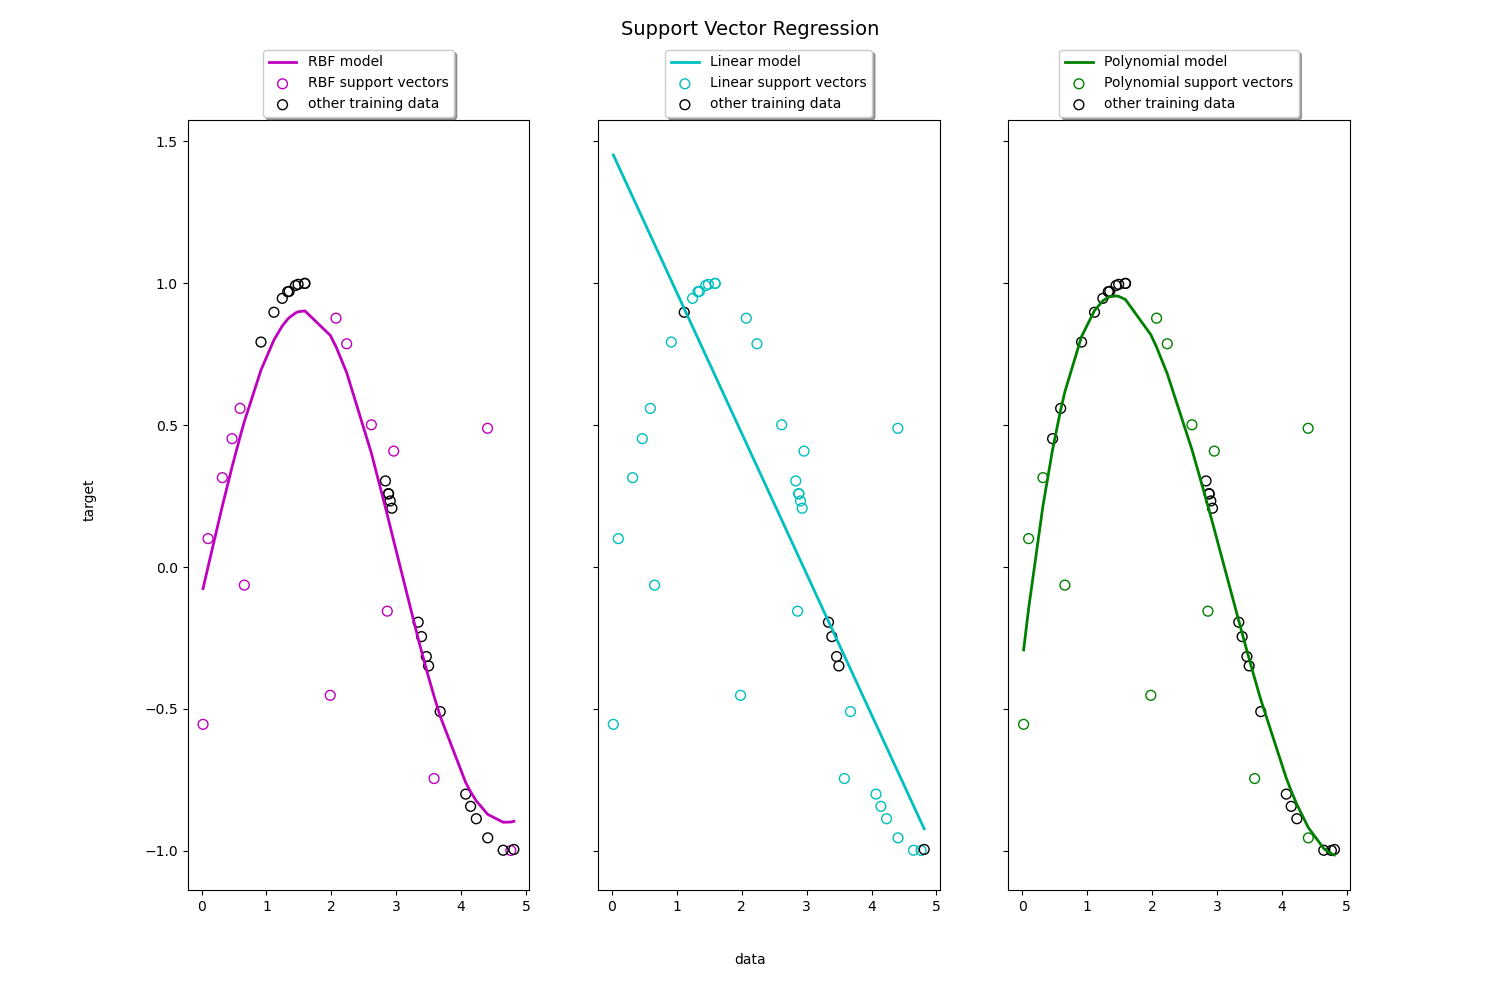
\includegraphics[width = 0.8\textwidth]{chapters/svm/images/svm_regression_cmp_models.png}
    \centering
    \caption{Сравнение SVM-регрессия с разными типами ядер}
    \label{fig:kernel_comparison}
\end{figure}

\subsection{Задача 1}
\textbf{Условие}:
\par Рассмотрим следующий набор точек, лежащих на границе \(\epsilon\) - окрестности для SVM-регрессии с линейным ядром:
\begin{equation*}
    \{(1, 2), (2, 3), (3, 5), (4, 6)\}
\end{equation*}
\par Постройте регрессионную модель и найдите смещение \(b\), если \(w = 2\), \(\epsilon = 1\).
\par \noindent \textbf{Решение:}
\par Для нахождения смещения \(b\) необходимо использовать точки, которые лежат на границах \(\epsilon\)-окрестности. Мы знаем, что для таких точек выполняется равенство:
\begin{equation*}
    y_i - (w x_i + b) = \epsilon \quad \text{или} \quad y_i - (w x_i + b) = -\epsilon
\end{equation*}
\par Найдем для каждой точки \(b\), подставив их координаты в эти уравнения:
\begin{itemize}
\item Для точки \((1, 2)\):
\begin{equation*}
    2 - (2 \cdot 1 + b) = 1 \quad \Rightarrow \quad 2 - (2 + b) = 1 \quad \Rightarrow \quad -b = 1 \quad \Rightarrow \quad b = -1
\end{equation*}
\item Для точки \((2, 3)\):
\begin{equation*}
    3 - (2 \cdot 2 + b) = 1 \quad \Rightarrow \quad 3 - (4 + b) = 1 \quad \Rightarrow \quad -b = 2 \quad \Rightarrow \quad b = -2
\end{equation*}
\item Для точки \((3, 5)\):
\begin{equation*}
    5 - (2 \cdot 3 + b) = 1 \quad \Rightarrow \quad 5 - (6 + b) = 1 \quad \Rightarrow \quad -b = 2 \quad \Rightarrow \quad b = -2
\end{equation*}
\item Для точки \((4, 6)\):
\begin{equation*}
    6 - (2 \cdot 4 + b) = 1 \quad \Rightarrow \quad 6 - (8 + b) = 1 \quad \Rightarrow \quad -b = 3 \quad \Rightarrow \quad b = -3
\end{equation*}
\end{itemize}
\par Для вычисления окончательного значения смещения \(b\), усредняем найденные значения:
\begin{equation*}
    b_{\text{avg}} = \frac{-1 + (-2) + (-2) + (-3)}{4} = \frac{-8}{4} = -2
\end{equation*}
\par Таким образом, смещение \(b = -2\).
\par Регрессионная модель для SVM с линейным ядром имеет следующий вид:
\begin{equation*}
    f(x) = w x + b
\end{equation*}
\par Подставляем данное в условии значения \(w = 2\) и найденное значение \(b = -2\):
\begin{equation*}
    f(x) = 2x - 2
\end{equation*}
\par Это и есть наша линейная регрессионная модель.
\par \noindent \textbf{Ответ:} \(f(x) = 2x - 2\).

\subsection{Задача 2}
\textbf{Условие:}
\par У нас есть два набора данных для задачи регрессии:
\begin{itemize}
    \item Набор 1: \( \{(1, 2), (2, 3), (3, 4), (4, 5)\} \)    
    \item Набор 2: \( \{(1, 1), (2, 4), (3, 9), (4, 16)\} \)  
\end{itemize}
\par Предположим, что мы используем SVM-регрессию с различными типами ядер (линейное, полиномиальное, RBF). Определите, какое ядро будет оптимальным для каждого набора данных.
\par \noindent \textbf{Решение:}
\begin{itemize}
    \item Набор 1: данные имеют линейную зависимость, следовательно, линейное ядро будет лучшим выбором.

    \item Набор 2: данные имеют квадратичную зависимость, следовательно, оптимально будет использовать полиномиальное ядро второй степени.
\end{itemize}
\par \noindent \textbf{Ответ:} для первого набора данных оптимальным ядром будет линейное, для второго набора данных - полиномиальное второй степени.

\subsection{Задача 3}
\textbf{Условие:}
\par Дан набор данных для SVM-регрессии с линейным ядром: 
\begin{equation*}
    \{(1, 2), (2, 2.8), (3, 5.2), (4, 8)\}.
\end{equation*}
\par Параметры модели: \(w = 1.5\), \(b = 0.5\), \(\epsilon = 0.5\). 
\begin{enumerate}
    \item Определите, какие из точек набора данных находятся вне \(\epsilon\)-окрестности (требуют штрафных переменных \(\xi\) или \(\xi^*\)).
    \item Вычислите значения штрафных переменных для этих точек.
\end{enumerate}
\par \noindent \textbf{Решение:}
\begin{enumerate}
\item Определение границ \(\epsilon\)-окрестности:
   Уравнение модели SVM-регрессии с линейным ядром: 
   \begin{equation*}
    f(x) = wx + b.
   \end{equation*}
   Подсталяем данные в условии значения:
   \begin{equation*}
    f(x) = 1.5x + 0.5.
   \end{equation*}
   Границы \(\epsilon\)-окрестности:
   \begin{equation*}
    f(x) - \epsilon \leq y \leq f(x) + \epsilon.
   \end{equation*}
\item Проверка точек:
\begin{itemize}
    \item Для точки \((1, 2)\): 
    \begin{equation*}
        f(1) = 1.5 \cdot 1 + 0.5 = 2.0, \quad 2 - 0.5 \leq 2 \leq 2 + 0.5 \quad (\text{в окрестности}).
    \end{equation*}
    \item Для точки \((2, 2.8)\): 
    \begin{equation*}
        f(2) = 1.5 \cdot 2 + 0.5 = 3.5, \quad 3.5 - 0.5 \not\leq 2.8 \leq 3.5 + 0.5 \quad (\text{вне окрестности}).
    \end{equation*}
    \item Для точки \((3, 5.2)\): 
    \begin{equation*}
        f(3) = 1.5 \cdot 3 + 0.5 = 5.0, \quad 5.0 - 0.5 \leq 5.2 \leq 5.0 + 0.5 \quad (\text{в окрестности}).
    \end{equation*}
    \item Для точки \((4, 8)\): 
    \begin{equation*}
        f(4) = 1.5 \cdot 4 + 0.5 = 6.5, \quad 6.5 - 0.5 \leq 8.0 \not\leq 6.5 + 0.5 \quad (\text{вне окрестности}).
    \end{equation*}
\end{itemize}
\item Штрафные переменные:
\begin{itemize}
    \item Для точки \((2, 2.8)\):
    \begin{equation*}
        \xi_i = f(2) - y - \epsilon = 3.5 - 2.8 - 0.5 = 0.2.
    \end{equation*}
    \item Для точки \((4, 8)\):
    \begin{equation*}
        \xi_i^* = y - f(4) - \epsilon = 8 - 6.5 - 0.5 = 1.0.
    \end{equation*}
\end{itemize}
Таким образом, штрафные переменные:
\begin{equation*}
    \xi_2^* = 0.2, \quad \xi_4 = 1.0.
\end{equation*}
\end{enumerate}
\par \noindent \textbf{Ответ:} \(\xi_2^* = 0.2, \quad \xi_4 = 1.0.\)


\setcounter{secnumdepth}{0}

\section{1-norm SVM (LASSO SVM)}
\subsection*{Аппроксимация эмпирического риска с \(L_1\)-регуляризацией}
\begin{align*}
    \sum_{i=1}^{\ell} \left(1 - M_i(w, w_0)\right)_+ + \mu \sum_{j=1}^{n} |w_j| & \rightarrow \min_{w, w_0}
\end{align*}

\subsection*{Плюс: отбор признаков с параметром селективности \(\mu\)}
\begin{itemize}
    \item чем больше \(\mu\), тем меньше признаков останется
\end{itemize}

\subsection*{Минус: слишком агрессивный отбор признаков}
\begin{itemize}
    \item по мере увеличения \(\mu\) признак может быть отброшен, хотя $y$ существенно зависит от него (даже когда ещё не все шумовые признаки отброшены)
\end{itemize}

\vspace{10pt}

\section{Сравнение L2 и L1 регуляризации}

Зависимость весов \(w_j\) от коэффициента \(\frac{1}{\mu}\):

\begin{itemize}
    \item \(L_1\) регуляризатор: \(\mu \sum_{j} |w_j|\)
\end{itemize}

\begin{figure}[ht]
    \centering
    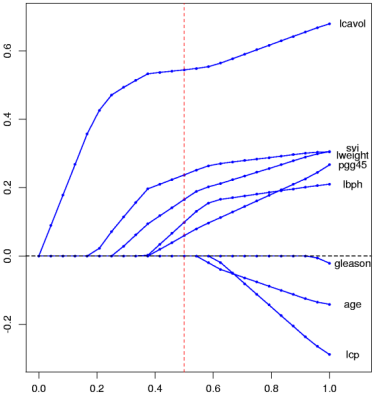
\includegraphics[width=0.6 \linewidth]{chapters/svm/images/L_1.png}
    \label{fig:image_1}    
\end{figure}

\begin{itemize}
    \item \(L_2\) регуляризатор: \(\mu \sum_{j} w_j^2\)
\end{itemize}

\begin{figure}[ht]
    \centering
    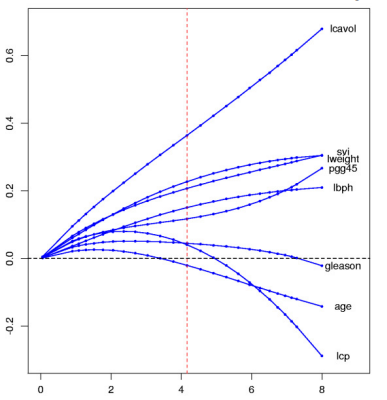
\includegraphics[width=0.6 \linewidth]{chapters/svm/images/L_2.png}
    \label{fig:image_2}    
\end{figure}

\section{Doubly Regularized SVM (Elastic Net SVM)}

\begin{align*}
    C \sum_{i=1}^{\ell} \left(1 - M_i(w, w_0)\right)_+ + \mu \sum_{j=1}^{n} |w_j| + \frac{1}{2} \sum_{j=1}^{n} w_j^2 & \rightarrow \min_{w, w_0}
\end{align*}

\subsection*{Плюсы:}
\begin{itemize}
    \item Параметр селективности \(\mu\) управляет отбором признаков: чем больше \(\mu\), тем меньше признаков останется
    \item Есть эффект группировки (grouping effect): значимые зависимые признаки отбираются вместе
\end{itemize}

\subsection*{Минусы:}
\begin{itemize}
    \item Шумовые признаки также группируются и могут вместе оставаться в модели
    \item Приходится подбирать два параметра регуляризации \(\mu, \tau\) (есть специальные методы, например, regularization path)
\end{itemize}

\subsection{Elastic Net Analysis}

Elastic Net менее жёстко отбирает признаки.

\begin{figure}[ht]
    \centering
    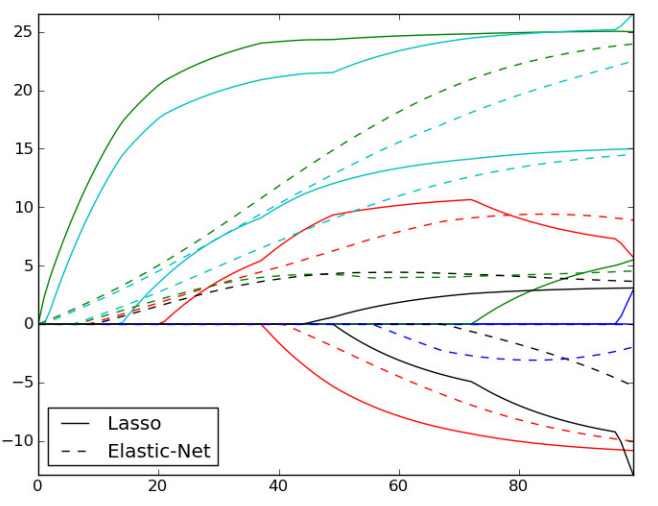
\includegraphics[width=0.8\linewidth]{chapters/svm/images/Elastic_Net.png}
    \caption{Зависимости весов \(w_j\) от коэффициента \(\log \frac{1}{\mu}\)}
    \label{fig:mpr}
\end{figure}

\section{Support Features Machine (SFM)}

\begin{align*}
    C \sum_{i=1}^{\ell} \left(1 - M_i(w, w_0)\right)_+ + \sum_{j=1}^{n} R_{\mu}(w_{j}) & \rightarrow \min_{w, w_0}
\end{align*}

\begin{align*}
R_{\mu}(w_j)=
    \begin{cases}
        2\mu |w_j|, & |w_j| \leq \mu\\
        \mu^2 + w_j^2, & |w_j| \geq \mu \\
    \end{cases}
\end{align*}

\subsection*{Плюсы}
\begin{itemize}
    \item Только один параметр регуляризации \(\mu\)
    \item Отбор признаков с параметром селективности \(\mu\)
    \item Эффект группировки: значимые зависимые признаки ($|w_j|$ > \(\mu\)) входят в решение совместно (как в $Elastic$ $Net$)
    \item Шумовые признаки ($|w_j|$ < \(\mu\)) не группируются и подавляются независимо друг от друга (как в $LASSO$)
\end{itemize}

\section{Relevance Features Machine (RFM)}

\begin{align*}
    C \sum_{i=1}^{\ell} \left(1 - M_i(w, w_0)\right)_+ + \sum_{j=1}^{n} \ln(w_j^2 + \frac{1}{\mu}) & \rightarrow \min_{w, w_0}
\end{align*}

\begin{align*}
    R(w) = \ln(w^2 + \frac{1}{\mu}), \quad \mu = 0.1, 1, 100
\end{align*}

\subsection*{Плюсы}
\begin{itemize}
    \item Только один параметр регуляризации \(\mu\)
    \item Отбор признаков с параметром селективности \(\mu\)
    \item Есть эффект группировки
    \item Лучше отбирает набор значимых признаков, когда они только совместно обеспечивают хорошее решение
\end{itemize}

\section{Задачи}

\subsection{Задача 1}

Качественно объяснить, почему $L_1$-регуляризатор приводит к отбору признаков

\subsection{Ответ:}

Аппроксимация эмпирического риска с \(L_1\)-регуляризацией:
\begin{align*}
    \sum_{i=1}^{\ell} \left(1 - M_i(w, w_0)\right)_+ + \mu \sum_{j=1}^{n} |w_j| & \rightarrow \min_{w, w_0}
\end{align*}

\textcolor{red}{Почему \(L_1\)-регуляризатор приводит к отбору признаков?}

Замена переменных: 
\[
u_j = \frac{1}{2} (|w_j| + w_j), \quad v_j = \frac{1}{2} (|w_j| - w_j).
\]
Тогда 
\[
w_j = u_j - v_j \quad |w_j| = u_j + v_j.
\]

\begin{align*}
    \sum_{i=1}^{\ell} \left(1 - M_i(u - v, w_0)\right)_+ + \mu \sum_{j=1}^{n} (u_j + v_j) & \rightarrow \min_{u, v}, \\
    u_j \geq 0, \quad v_j \geq 0, \quad j = 1, \ldots, n.
\end{align*}

чем больше \(\mu\), тем больше индексов \(j\) таких, что \(u_j = v_j = 0\), но тогда \(w_j = 0\), значит, \textcolor{red}{признак не учитывается.}

\subsection{Задача 2}

Привести пример нежелательного эффекта в процессе обучения, с которым поможет справиться регуляризация 
 
\subsection{Ответ:}

Регуляризация помогает в случае линейной зависимости (мультиколлинеарности) признаков:\\
Пусть построен классификатор: $a(x, w) = sign\langle w, x \rangle$ \\
Мультиколлинеарность: $\exists$  $u \in \mathbb{R}^{n}$: $\forall x \in X$ $\langle u, x \rangle = 0$ \\
Неединственность решения и рост нормы вектора весов: $\forall \gamma \in \mathbb{R}$ $a(x, w) = sign\langle w, x \rangle = sign \langle w + \gamma u, x \rangle$ \\
\\
Проявления переобучения:
\begin{itemize}
    \item слишком большие веса $|w_j|$ разных знаков
    \item неустойчивость дискриминантной функции $\langle w, x \rangle$
    \item $Q(X^{\ell}) \ll Q(X^{k})$
\end{itemize}
Способ уменьшить переобучение:\\
регуляризация $||w|| \rightarrow min$ (сокращение весов, $weight$ $decay$)

\subsection{Задача 3}

Дана задача оптимизации:
\begin{align*}
    \frac{1}{2}(wx - b)^2 + \lambda|w| & \rightarrow \min_{w},
\end{align*}
где $x,$ $b$ $\in \mathbb{R};$ $\lambda \geq 0$\\
При каких $\lambda$ данная задачи имеет решение $w_0 \neq 0?$
 
\subsection{Ответ:}

Находим правую и левую односторонние производные в нуле и рассматриваем, когда они больше и меньше 0 соответственно:

\begin{align*}
    \begin{cases}
        -xb + \lambda > 0\\
        -xb - \lambda < 0\\
        \lambda \geq 0\\
    \end{cases} \Leftrightarrow \lambda > |xb|
\end{align*}

Это условие на $\lambda,$ при котором задача имеет решение $w_0 = 0,$ поэтому нам подходит $\lambda \in [0;$ $|xb|)$.


\section{Ядерные функции машины опорных векторов}
При наличии нелинейной связи между признаками и откликом качество линейных классификаторов, как показано на рисунке ниже,
часто может оказаться неудовлетворительным.
\begin{align*}
    \centering
    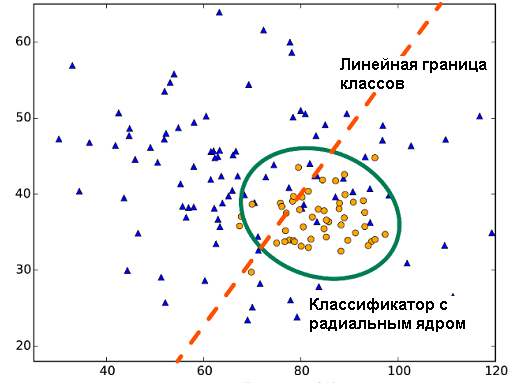
\includegraphics[width=0.6 \linewidth]{chapters/svm/images/svm_kernels.png}
    \label{fig:image}
\end{align*}
Для учета нелинейности обычно расширяют пространство переменных,
включая различные функциональные преобразования исходных предикторов (полиномы, экспоненты и проч.).
Машину опорных векторов SVM (Support Vector Machine) можно рассматривать как нелинейное обобщение линейного классификатора, полученного при
решении двойственной задачи (прямая задача является задачей бинарной классификации):
$$
\left\{\begin{array}{l}
w=\sum_{i=1}^{\ell} \lambda_i y_i x_i ; \\
w_0=\left\langle w, x_i\right\rangle-y_i, \quad \text { для любого } i: \lambda_i>0, M_i=1 .
\end{array}\right.
$$

Линейный классификатор с признаками $f_i(x)=\left\langle x, x_i\right\rangle$ :
$$
a(x)=\operatorname{sign}\left(\sum_{i=1}^{\ell} \lambda_i y_i\left\langle x, x_i\right\rangle-w_0\right) .
$$

Введя здесь новую нелинейную функцию $K\left(x, x^{\prime}\right)$, вместо $\left\langle x, x^{\prime}\right\rangle$,
можно строить модели с разделяющих поверхностями самой различной формы.

Дадим формальное определение:\newline
\textbf{Oпределение}:\newline
Функция $K: X \times X \rightarrow \mathbb{R}-$ ядро, если $K\left(x, x^{\prime}\right)=\left\langle\psi(x), \psi\left(x^{\prime}\right)\right\rangle$
при некотором $\psi: X \rightarrow H$, где $H-$ гильбертово пространство. \newline
В качестве таких функций чаще всего используют следующие:
\begin{itemize}
\item линейное ядро: $K(x, x^{\prime})=\langle x, x^{\prime} \rangle$, что соответствует классификатору на опорных векторах в исходном пространстве (см. рис. 6.3);
\item полиномиальное ядро со степенью $p: K(x, x^{\prime})=(1+\langle x, x^{\prime} \rangle)^p$;
\item гауссово ядро с радиальной базовой функцией (RBF): $K(x, x^{\prime})=\exp(\gamma\langle x - x^{\prime} \rangle^2)$;
\item сигмодиное ядро: $K(x, x^{\prime})=\tanh(\gamma\langle x, x^{\prime}\rangle+\beta_0)$.
\end{itemize}

Для того, чтобы определять является ли функция ядром, существует\newline
\textbf{Теорема Мерсера}:\newline
Функция двух переменных $K\left(x, x^{\prime}\right)$ является ядром тогда и только тогда, когда она
\begin{itemize}
\item симметрична, то есть $K\left(x, x^{\prime}\right)=K\left(x^{\prime}, x\right)$;
\item неотрицательно определена, то есть $\int_X \int_X K\left(x, x^{\prime}\right) g(x) g\left(x^{\prime}\right) d x d x^{\prime} \geq 0$ для любой функции $g: X \rightarrow \mathbb{R}$;
\end{itemize}

Нужно отметить, что на практике проверка неотрицательной определенности функции $K\left(x, x^{\prime}\right)$ часто является нелегкой задачей.
Вместо этого обычно используют какие-то конструктивные методы синтеза ядер, например достаточно очевидное утверждение: $K\left(x, x^{\prime}\right)=\alpha_1 K_1\left(x, x^{\prime}\right)+\alpha_2 K_2\left(x, x^{\prime}\right)$ при $\alpha_1, \alpha_2>0-$ ядро.

\subsection{Задача 1}
Найти пространство $H$ и преобразование $\psi: X \rightarrow H$, при которых
$K(x, x^{\prime}) = \langle \psi(x),\psi(x^{\prime}) \rangle $, где $X = \mathbb{R}^n,~
K(x, x^{\prime}) = \langle x, x^{\prime} \rangle^2,~ x = (x_1, x_2, \cdots x_n),~ x^{\prime} = (x_1^{\prime}, x_2^{\prime}, \cdots x_n^{\prime})$
\subsection{Решение}
\begin{align*}
K(x, x^{\prime}) = \langle x, x^{\prime} \rangle^2 = \langle (x_1, x_2, \cdots x_n), (x_1^{\prime}, x_2^{\prime}, \cdots x_n^{\prime}) \rangle^2 = (x_1x_1^{\prime} + \cdots + x_nx_n^{\prime})^2  \\
  = x_1^2x_1^{\prime}^2 + \cdots + \cdots x_n^2x_n^{\prime}^2 + 2x_1x_1^{\prime}x_2x_2^{\prime} + \cdots 2x_1x_1^{\prime}x_{n}x_n^{\prime} + \cdots + 2x_{n-1}x_{n-1}^{\prime}x_{n}x_{n}^{\prime}  = \\
  = \langle(x_1^2, x_2^2, \cdots x_n^2, \sqrt{2}x_1x_2, \cdots \sqrt{2}x_{n-1}x_n),(x_1^{\prime}^2, x_2^{\prime}^2, \cdots x_n^{\prime}^2, \sqrt{2}x_1^{\prime}x_2^{\prime},\cdots \sqrt{2}x_{n-1}^{\prime}x_{n}^{\prime})\rangle
\end{align*}
Подсчетом слагаемых можно убедиться, что $ dimH = \frac{1}{2}n(n-1) $, а $\psi:(x_1, x_2, \cdots x_n) \mapsto(x_1^2, x_2^2, \cdots x_n^2, \sqrt{2}x_1x_2, \cdots \sqrt{2}x_{n-1}x_n)$

\subsection{Задача 2}
Доказать, что $\forall \psi: X \rightarrow \mathbb{R}$ произведение $K\left(x, x^{\prime}\right)=\psi(x) \psi\left(x^{\prime}\right)-$ ядро.
\subsection{Решение}

Действительно, произведение $\psi(x) \psi(x^{\prime})$ есть скалярное произведение в одномерном пространстве $\mathbb{R}$, а в силу свойств скалярного произведения
(положительная определенность и симметричность) по теореме Мерсера получаем, что $K(x, x^{\prime})$ ядро.

\subsection{Задача 3}
Доказать, что $K(x, x^{\prime})=\exp(\langle x - x^{\prime} \rangle^2)$ ядро (гауссово ядро с радиальной базовой функцией).
\subsection{Решение}

Для доказательство нужно воспользоваться утверждением: композиция произвольного ядра $K_0$ и произвольной функции
$f: \mathbb{R} \rightarrow \mathbb{R}$, представимой в виде сходящегося степенного ряда с неотрицательными коэффициентами
$K\left(x, x^{\prime}\right)=f\left(K_0\left(x, x^{\prime}\right)\right)$, является ядром.
$K_0(x, x^{\prime}) = \langle x - x^{\prime} \rangle^2$ является ядром по свойствам скалярного произведения. Как известно,
экспонента представима в виде степенного ряда с положительными коэффициентами, поэтому выполнены все условия утверждения, что
доказывает, что $K(x, x^{\prime})$ ядро.


\section{Relevance Vector Machine(RVM)}

\subsection{Идея метода релевантных векторов}

Берем за основу структуру решения как в SVM:\\
\begin{align*}
   \sum_{i=1}^{\ell} \lambda_i y_i x_i
\end{align*}

(опорным векторам $x_i$ соответствуют $\lambda_i \neq 0$) \\
\textbf{Проблема:} Какие из коэффициентов $\lambda_i$ лучше обнулить? \\
Делаем так, что регуляризатор зависит не от w, а от $\lambda_i$. \\
\begin{align*}
       \rho (\lambda) = \frac{1}{(2\pi)^{l/2} \sqrt{\alpha_1...\alpha_l}} exp(-\sum_{i=1}^{\ell} \frac{\lambda_i^2}{2\alpha_i})
\end{align*}
- т.е. $\lambda_i$ - независимые, гауссовские и с дисперсиями $\alpha_i$ \\
Будем решать задачу оптимизации с регуляризатором (логарифмируем плотность - дисперсию не считаем константой): \\
\begin{align*}
       \frac{1}{2} \sum_{i=1}^{\ell} ln\alpha_i + \frac{\lambda_i^2}{\alpha_i}
\end{align*} 
Задача оптимизации:  \\
\begin{align*}
       \sum_{i=1}^{\ell} (1 - M_i(w(\lambda), w_0))_+ + \frac{1}{2} \sum_{i=1}^{\ell} ln\alpha_i + \frac{\lambda_i^2}{\alpha_i} \rightarrow \min_{\lambda, \alpha}
\end{align*}
Если одновременно оптимизируем и $\lambda$ и $\alpha$, то при уменьшении дисперсию, $\lambda$ будет маленькая - то есть "обнуляться" и соответствующие объекты не будут опорными. 

\subsection*{Плюсы}
\begin{itemize}
    \item Опорных векторов, как правило меньше (более "разреженное" решение)
    \item Шумовые вабросы уже не входят в число опорных
    \item Не надо искать параметр регуляризации (вместо этого $\alpha_i$ оптимизируется в процессе обучения)
    \item Аналогично SVM, можно использовать ядра
\end{itemize}

\subsection*{Минусы}
\begin{itemize}
    \item Не всегда есть преимущество по качеству классификации
\end{itemize}

\subsection{Задачи по RVM}
\textbf{Задача 1:}\\
Объяснить, как метод релевантных векторов (Relevance Vector Machine, RVM) достигает разреженности в параметрах модели.  \\
\textbf{Ответ:}\\
Метод релевантных векторов (RVM) достигает разреженности через байесовскую структуру, устанавливая независимые нормальные априорные распределения с нулевым средним для весов модели, каждый с собственной гиперпараметром точности (обратная дисперсия). Конкретно, для каждого веса $w_i$ существует связанный гиперпараметр точности $\alpha_i$. 
Априорное распределение весов задается как:\\
Априорное распределение весов задается как:
\begin{align*}
       p(\mathbf{w} | \boldsymbol{\alpha}) = \prod_{i=1}^N \mathcal{N}(w_i | 0, \alpha_i^{-1})
\end{align*}

В процессе обучения RVM определяет гиперпараметры  $\boldsymbol{\alpha} = [\alpha_1, \alpha_2, \dots, \alpha_N]$, максимизируя маржинальное правдоподобие данных. Многие из этих гиперпараметров стремятся к бесконечности, что приводит к обнулению соответствующих весов $ w_i$. 

\textbf{Задача 2:}\\
Объяснить, в чем заключается основное отличие метода релевантных векторов (RVM) от метода опорных векторов (SVM), если рассматривать их с точки зрения подхода к регуляризации и использования априорных предположений. \\
\textbf{Ответ:}
\begin{itemize}
    \item Основное отличие заключается в том, что RVM использует байесовский подход, тогда как SVM — детерминированный метод. 
    \item В RVM вводятся априорные распределения на веса модели, что позволяет автоматически выполнять регуляризацию, оставляя наиболее значимые параметры.
    \item В результате RVM достигает разреженности (аналогично SVM) без использования параметра регуляризации, а лишь за счет максимизации апостериорной вероятности.

\end{itemize}


\textbf{Задача 3:}\\
Объяснить, в чем метод релевантных векторов может быть быстрее и медленнее метода опорных векторов \\
\textbf{Ответ:} \\
\textbf{Быстрее, потому что:}
 \begin{itemize}
    \item В RVM гораздо быстрее применение модели к новым точкам, потому что опорных векторов гораздо меньше 
    \item В SVM необходимо оптимизировать параметр регуляризации C (или аналогичный параметр для других ядер), что требует дополнительных затрат времени. В RVM регуляризация происходит автоматически через байесовский подход (гиперпараметры $\alpha_i$), устраняя необходимость выбора таких параметров вручную.

\end{itemize}
\textbf{Медленнее, потому что:}
\begin{itemize}
    \item Байесовский подход в RVM делает процесс обучения более ресурсоемким, чем у SVM. Это связано с итеративными расчетами для апостериорных вероятностей и гиперпараметров - обучение происходит дольше
\end{itemize}

\section{Резюме по линейным классификаторам}
\begin{itemize}
    \item SVM - лучший метод линейной классификации
    \item SVM изящно обобщается для нелинейной классификации, для линейной и нелинейной регрессии
    \item Аппрксимация пороговой функции потерь $\L (M)$ увеличивает зазор и повышает качество классификации
    \item Регуляризация устраняет мультиколлинеарность и уменьшает переобучение
    \item Негладкость функции потерь приводит к отбору объектов
    \item Негладкость регуляризатора приводит к отбору признаков
\end{itemize}
\textbf{Комментарий по последним двум пунктам:} \\
Отбор опорных объектов возник из-за того, что возникает негладкая функция потерь, аналогично (но смотрим с другой стороны)  отбор признаков так же связан с негладкостью регуляризатора. \\
Что мы можем отбирать в задаче классификации? \\
У нас есть матрица объекты - признаки, то есть либо строки, либо столбцы являются лишними.\\ Cоответственно и возникает подход: решаем задачу классификации, отфильтровав матрицу по строкам и по столбцам. \\
Фильтрация может быть реализована:
\begin{itemize}
    \item путем выбора негладких функций потерь, которые приводят к фильтрации строк (набора объектов)
    \item путем выбора негладких регуляризаторов, которые приводят к фильтрации столбцов (набора признаков)
\end{itemize}
Роль регуляризации возникает благодаря выписыванию оптимизационной задачи с ограничениями-неравенствами $\rightarrow$ требуется применять условие Каруша-Куна-Таккера (применимы только к гладким функциям) \\ 
Если функция негладкая $\rightarrow$ вводим дополнительные переменные, неотрицательные и могут обращаться в ноль $\rightarrow$ происходит отбор \\


\section{Обобщения линейного SVM. Ядра и спрямляющие пространства. SVM как двухслойная нейронная сеть.}
\subsection*{Нелинейное обобщение SVM}
\textbf{Определение}. Функция $K: X \rightarrow X$ - ядро, если $K(x, \tilde{x}) = \langle \psi, \tilde{\psi} \rangle $ при некотором $\psi: X \rightarrow H$, где $H$ - гильбертово пространство

\noindent\textbf{Теорема}. Функция $K(x, \tilde{x})$ является ядром тогда и только тогда, когда
она симметрична: $K(x, \tilde{x}) = K(\tilde{x}, x)$ и неотрицательно определена:
$ \iint\limits_{XX} K(x, \tilde{x})g(x)g(\tilde{x}) dxdy \ge 0$ для любой $g: X \rightarrow \mathbb{R}$

\noindent\textbf{Конструктивные методы синтеза ядер:}
\begin{itemize}
  \item $K(x, \tilde{x}) = \text{\textlangle} x, \tilde{x} \text{\textrangle} ~$ - ядро
  \item $K(x, \tilde{x}) = 1$ - ядро
  \item $K(x, \tilde{x}) = K_1(x, \tilde{x}) \times K_2(x, \tilde{x})$ - ядро, если $K_1, K_2$ - ядра
  \item $K(x, \tilde{x}) = \psi(x)\psi(\tilde{x})$ - ядро при $\psi: X \rightarrow \mathbb{R}$
  \item $K(x, \tilde{x}) = \alpha_1 K_1(x, \tilde{x}) + \alpha_2 K_2(x, \tilde{x}), ~ \alpha_1 > 0, \alpha_2 > 0$
  \item $K(x ,\tilde{x}) = \iint\limits_{X} s(x, z) s(\tilde{x}, z) dz$ - ядро, если $s: X \times X \rightarrow \mathbb{R}$ - симметричная интегрируемая функция
  \item $K(x, \tilde{x}) = f(K_0(x, \tilde{x}))$ - ядро, если $K_0$ - ядро и $f: \mathbb{R} \rightarrow \mathbb{R}$ представима в виде сходящегося степенного ряда с неотрицательными коэффицентами 
\end{itemize}

\subsection{Задача 1}
Найти пространство $H$ и преобразование $\psi: X \rightarrow H$, при которых 
$K(x, \tilde{x}) = \langle \psi(x),\psi(\tilde{x}) \rangle $, где $X = \mathbb{R}^2,~
K(u, v) = \langle u, v \rangle^2,~ u = (u_1, u_2),~ v = (v_1, v_2)$
\subsection{Решение}
\begin{align*}
  K(u, v) = \langle u, v \rangle^2 = \langle (u_1, u_2), (v_1, v_2) \rangle^2 = (u_1v_1 + u_2v_2)^2 = u_1^2 u_2^2 + 2u_1v_1u_2v_2 = \\
  = \langle(u_1^2, u_2^2, \sqrt{2}u_1u_2),(v_1^2, v_2^2, \sqrt{2}v_1v_2)\rangle 
\end{align*}
То есть $ H = \mathbb{R}^3, ~ \psi: (u_1, u_2) \rightarrow (u_1^2, u_2^2, \sqrt{2}u_1u_2)$

\subsection{Задача 2}
Решите предыдущую задачу при условии, что $X = \mathbb{R}^n, ~ K(u, v) = \langle u, v \rangle^{d}$
\subsection{Решение}
Заметим, что в таком случае компонентами вектора $\psi(u)$ будут различные произведения $(u_1)^{d_1}, (u_2)^{d_2}, ..., (u_n)^{d_n}~$ при
$d_1, d_2, ..., d_n: d_1 \ge 0, d_2 \ge 0, ..., d_n \ge 0$ и $ d_1 + d_2 + ... + d_n = d$. Число мономов и есть размерность пространства $H$: $dim H = C_{n + d - 1} ^ d$ - число сочетаний с повторением.

\subsection{Задача 3}
Представьте нелинейное обобщение SVM для классификатора в виде двухслойной нейронной сети. Считать,
что опорные объекты из множества $ X = \mathbb{R}^n~$
\subsection{Решение}
Обозначим $x_1, x_2, ..., x_h$ как опорные объекты. Тогда
\begin{align}
  a(x) = sign(\sum_{i = 1}^{h} \lambda_i y_i K(x, \tilde{x}) - w_0)
\end{align}

\noindent Двухслойная нейронная сеть представлена на рисунке ниже.

\begin{figure}[h!]
  \centering
  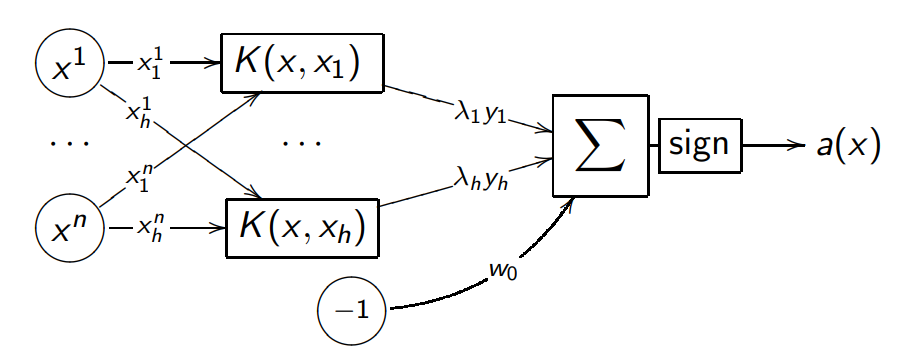
\includegraphics[width=0.8\linewidth]{chapters/svm/images/SVM_neuron.png}
  \caption{SVM в виде двухслойной нейросети}
  \label{fig:mpr}
\end{figure}
